\chapter{Платформа для проведения виртуального эксперимента} \label{chapt4}


\section{Архитектура платформы}\label{sect_4_2}
В данном разделе рассмотрены архитектура платформы (\cref{fig:arch}) и то, каким образом компоненты архитектуры 
поддерживают различные этапы деятельности эксперта по проведению виртуальных экспериментов 
\cite{kovalev2020architecture}. 
На рисунке пунктирные стрелки обозначают доступ из одного компонента к интерфейсу другого компонента. Программная 
архитектура системы исполнения виртуального эксперимента включает в себя компоненты, поддерживающие различные этапы 
проведения виртуальных экспериментов. В настоящее время архитектура находится в стадии программной реализации.

Разработанный в рамках проекта прототип системы управления виртуальными экспериментами нацелен на объединение 
преимуществ и преодоление недостатков существующих систем. На основании анализа предметной области управления 
виртуальными экспериментами и родственных работ формализовано общее понятие виртуального эксперимента, включающее 
онтологию предметной области, набор спецификаций гипотез и взаимосвязей между ними, набор моделей, реализующих 
гипотезы, поток работ, реализующий эксперимент, конфигурацию (набор значений параметров) эксперимента. Сформулированы 
общие требования к системе для управления виртуальными экспериментами, которым удовлетворяет реализованный прототип. 
Отслеживается эволюция моделей, гипотез и экспериментов. На основании анализа методов формального манипулирования 
виртуальными экспериментами и гипотезами при сохранении непротиворечивости экспериментов для систем с явным 
представлением и использованием гипотез выбраны и реализованы операции управления виртуальными экспериментами и 
их составляющими (гипотезы, модели, их конфигурации). Реализованы методы ранжирования конкурирующих гипотез по 
соответствию наблюдаемым данным на одном или нескольких наборах данных. Предоставляются структуры для хранения 
результатов предыдущих экспериментов, и обеспечиваются запросы к ним. Реализован метод автоматизированного построения 
решеток причинно-следственных зависимостей гипотез в виртуальных экспериментах. Реализован метод порождения гипотез 
из данных, сочетающий обобщенную линейную модель, генетическое программирование и динамическое причинно-следственное 
моделирование. Разработаны и реализованы метод поиска оптимальных параметров гипотез и метод корректной оценки 
соответствия гипотезы исследуемому явлению. Реализован метод повышения эффективности и скорости проведения виртуальных 
экспериментов. Реализованы методы сравнения конкурирующих гипотез, построенных из данных, с теоретическими гипотезами 
из теоретического моделирования или литературы. Реализован подход к интеграции экспериментов, гипотез и данных с 
данными новых наблюдений, симуляций и метаданных экспериментов.

Компонент MetadataRepository представляет собой репозиторий метаинформации (базу данных), предназначенный для хранения 
результатов выполнения виртуального эксперимента с учетом накопления данных о добавлении, модификации и удалении 
гипотез, потоков работ, онтологий и виртуальных экспериментов. Дополнительно в репозитории сохраняются построенные 
зависимости между гипотезами (полученными либо от эксперта, либо автоматически извлеченные) и имеющейся информации 
о корреляции между параметрами как в рамках одной, так и параметров нескольких гипотез.

\begin{figure}[h!]
    \centering
    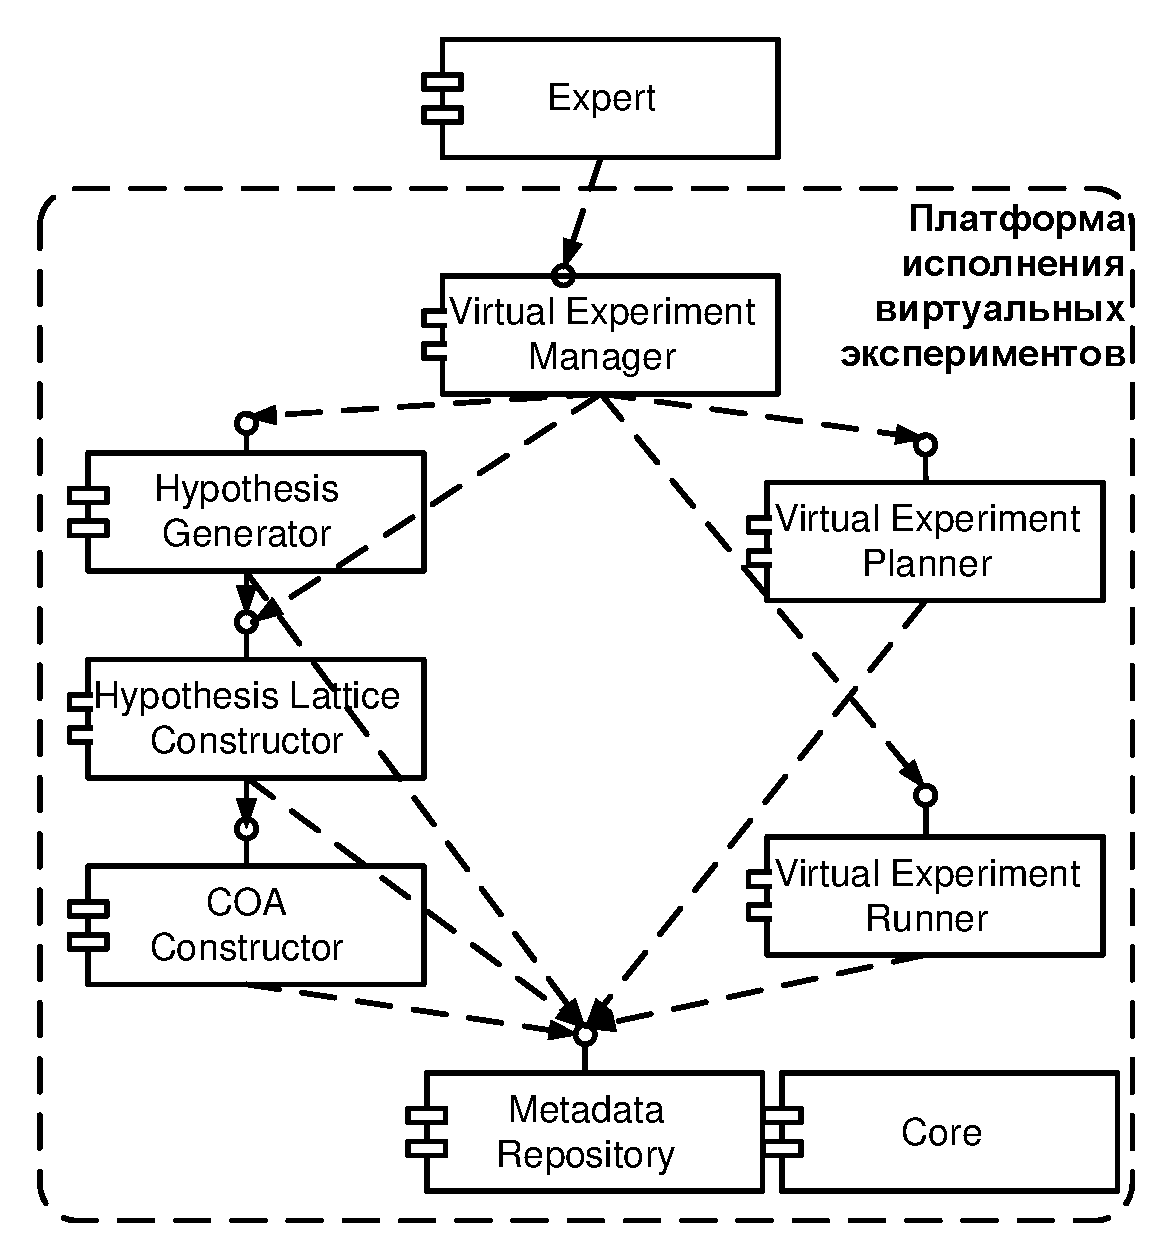
\includegraphics[width=0.7\linewidth]{images/arch_v4.pdf}
    \caption{Архитектура платформы исполнения виртуальных экспериментов.}\label{fig:arch}
\end{figure}

\subsection{Ядровой компонент}
В данном разделе приведено описание ядрового компонента платформы исполнения виртуального эксперимента.
В компоненте представлены методы, которые описывают реализацию подходов из раздела 2 и 
на рис. \cref{fig:core_hypothesis}. 

\begin{figure}[ht]
    \centering
    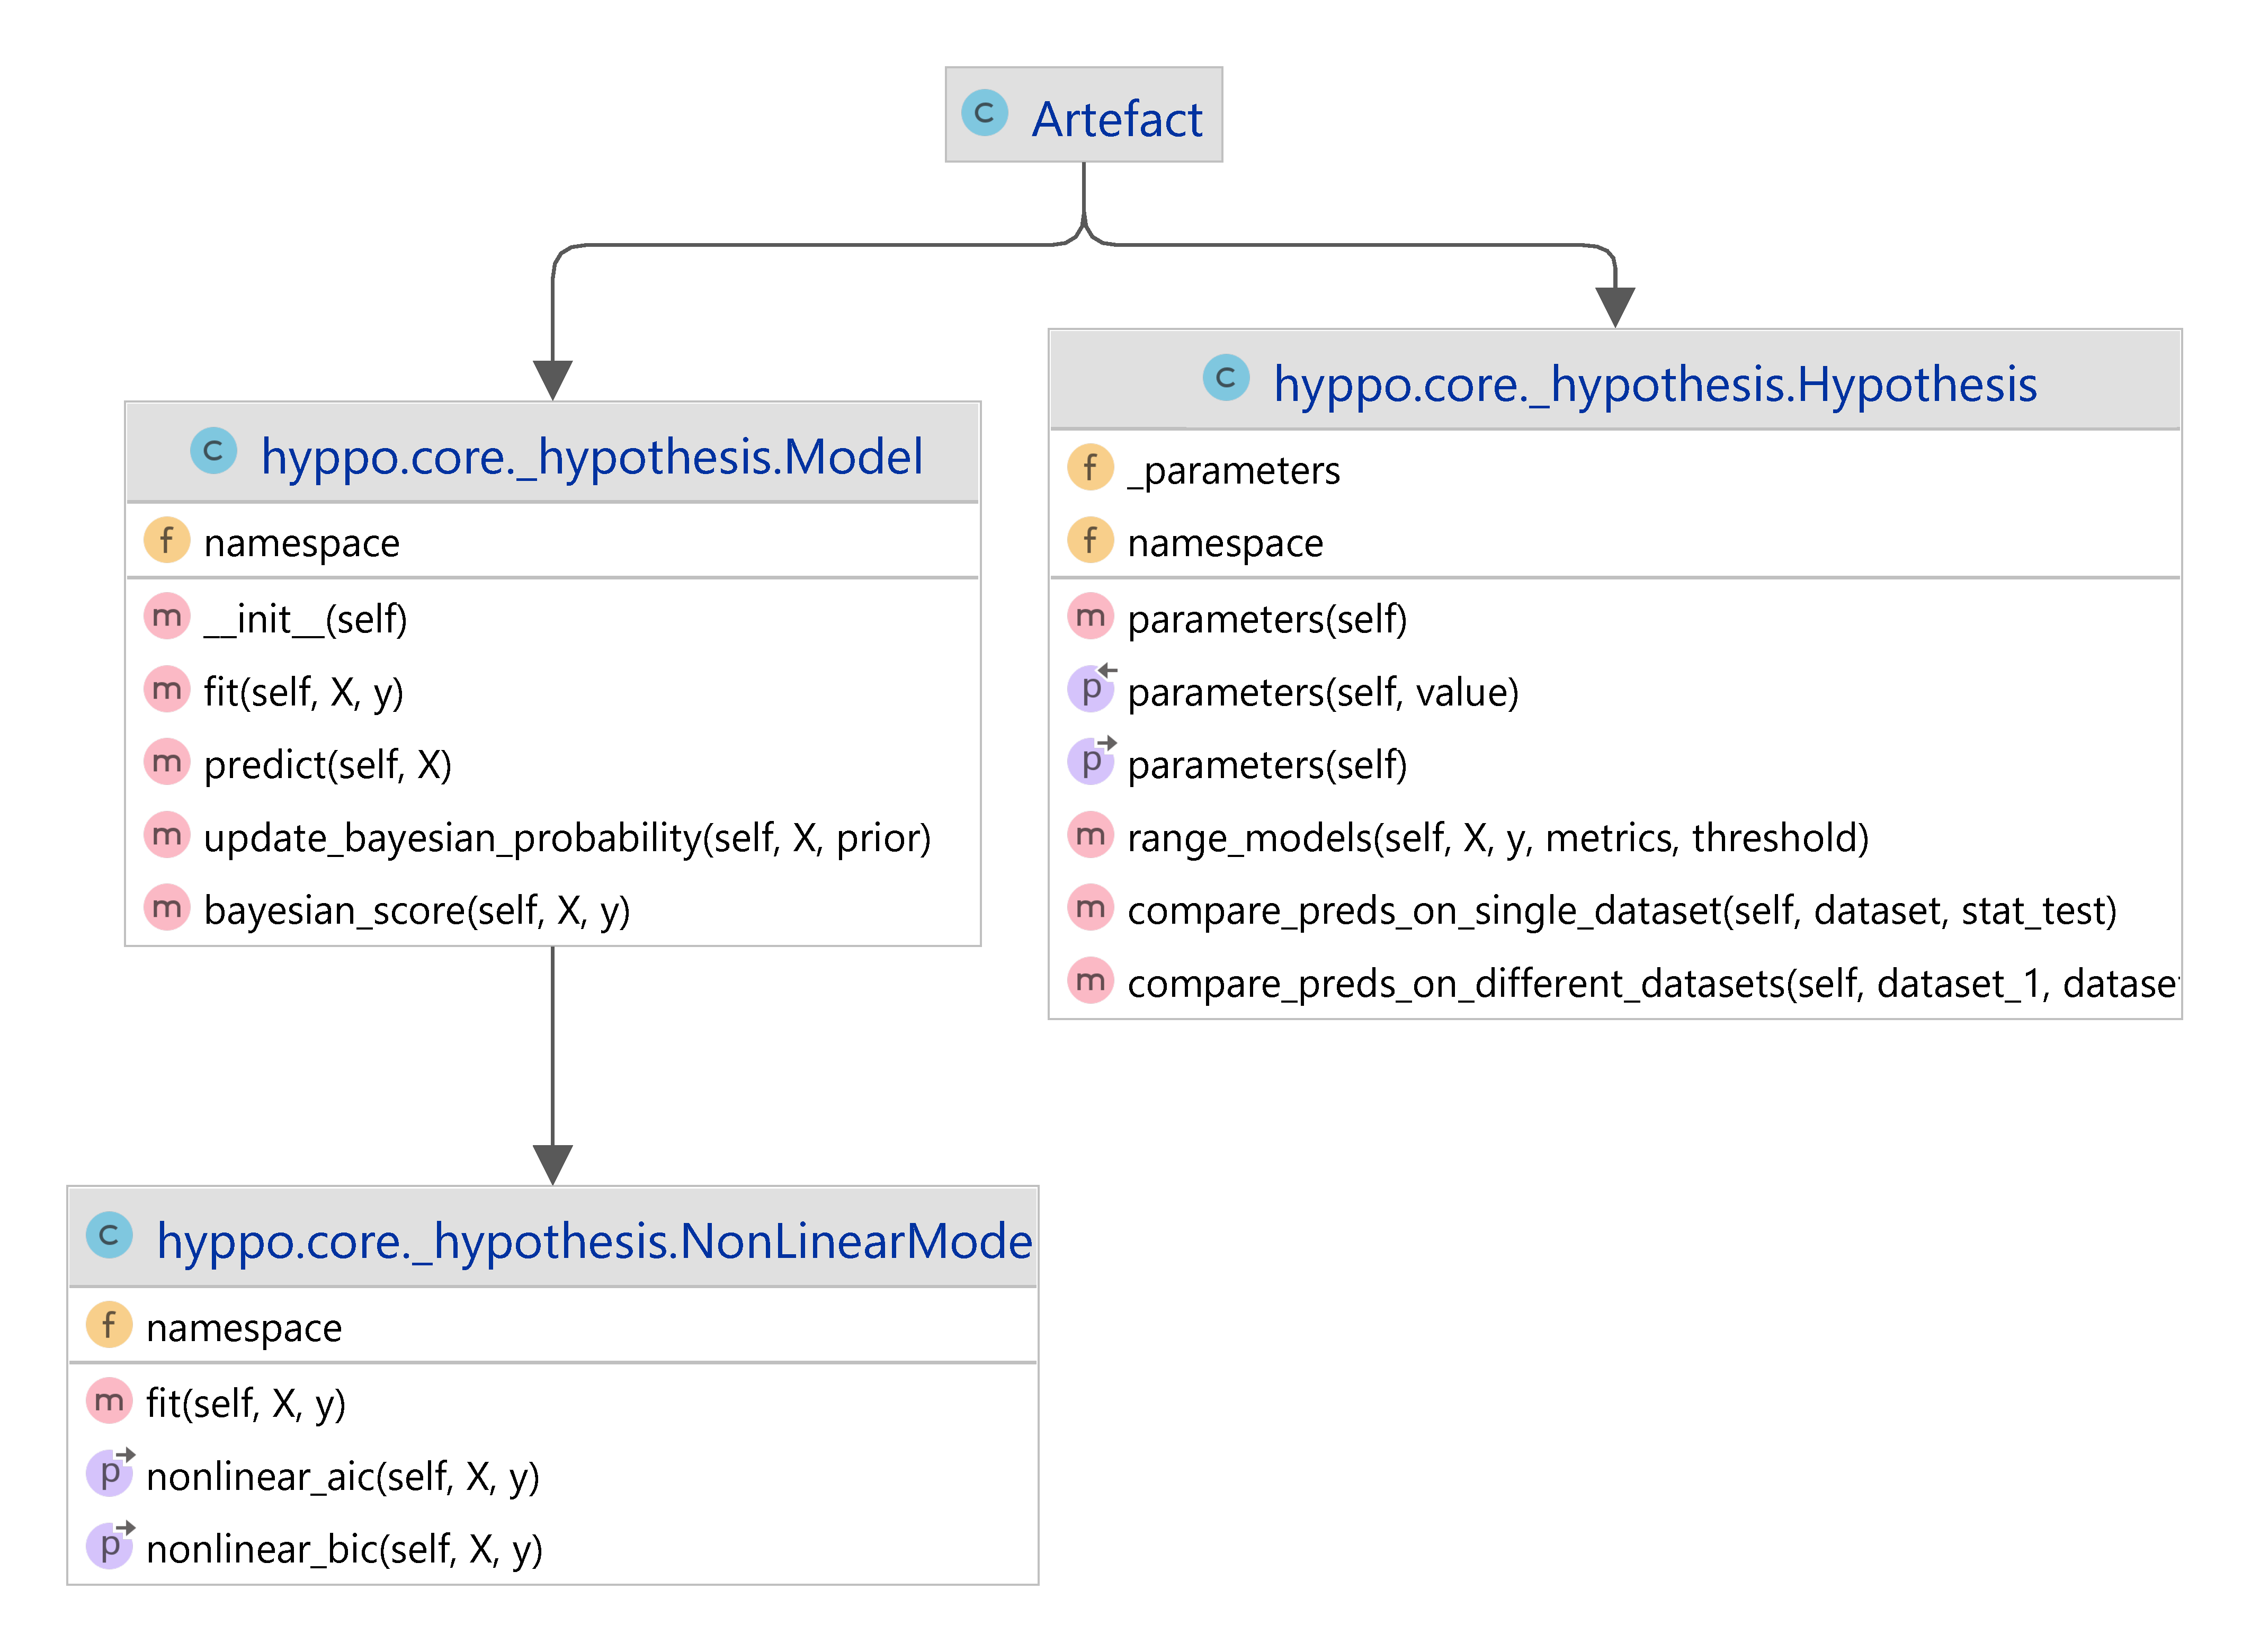
\includegraphics[width=0.7\linewidth]{images/_hypothesis.pdf}
    \caption{Гипотезы и модели в ядровом компоненте.}\label{fig:core_hypothesis}
\end{figure}

\begin{itemize}
   
\item \textit{range\_models(models, dataset, metrics, threshold)} "--- метод для ранжирования моделей по выбранной 
        метрике на выбранном наборе данных. На вход метод принимает набор моделей, которые требуется ранжировать, 
        набор данных, на котором строится выбранная метрика, метрику предсказаний, порог значений для отсечения 
        плохих моделей. В качестве метрик предсказаний могут быть использованы метрики из библиотеки sklearn, 
        например, среднеквадратичную ошибку или коэффициент детерминации, а также информационные критерии, 
        определенные ниже. На выходе метод возвращает ранжированный список моделей с вычисленными метриками.
\item \textit{get\_AIC(model, dataset)} "--- построение информационного критерия Акаике для выбранных модели и набора 
        данных. На вход метод принимает модель и набор данных, на выходе возвращает информационный критерий Акаике.
\item \textit{get\_BIC(model, dataset)} "--- построение Байесовского информационного критерия для выбранных модели и 
        набора данных. На вход метод принимает модель и набор данных, на выходе возвращает 
        Байесовский информационный критерий.
\item \textit{get\_AIC\_nonlinear(model, dataset)} "--- построение информационного критерия Акаике для выбранных 
        нелинейной модели и набора данных. На вход метод принимает модель и набор данных, на выходе возвращает 
        информационный критерий Акаике для нелинейной модели.
\item \textit{get\_BIC\_nonlinear(model, dataset)} "--- построение Байесовского информационного критерия для выбранных 
        нелинейной модели и набора данных. На вход метод принимает модель и набор данных, на выходе возвращает 
        Байесовский информационный критерий для нелинейной модели.
\item \textit{update\_bayesian\_probability(model, dataset, prior\_probability)} "--- метод по построению Байесовской 
        вероятности для выбранной модели на выбранном наборе данных с учетом заданной априорной оценки вероятности. 
\item \textit{compute\_bayesian\_hypotheis\_score(model, dataset)} "--- метод по вычислению байесовской оценки 
        соответствия предсказаний модели наблюдениям.
\item \textit{compare\_models(models, dataset, stattest)} "--- метод сравнения двух моделей между собой на одном 
        наборе данных. На вход метод принимает две модели, набор данных, а также выбранный экспертом статистический 
        тест. На выходе метод возвращает истину, если нельзя отбросить гипотезу о 
        различии предсказаний моделей, иначе ложь. 
\item \textit{compare\_preds\_on\_diff\_sets(models, dataset\_1, dataset\_2, stattest)} "--- метод сравнения моделей 
        между собой на двух наборе данных. На вход метод принимает модель, два набора данных, а также выбранный 
        экспертом статистический тест. На выходе метод возвращает истину, если нельзя отбросить гипотезу о различии 
        предсказаний модели, иначе ложь.
\item \textit{compute\_diff\_dag(models, dataset)} "--- метод для вычисления графа разности двух ориентированных 
        ацикличных графов, построенных по данным входных моделей. На входные модели налагается 
        дополнительное ограничение о линейности. На выходе метод возвращает вычисленный граф разности моделей. 
        Если множество ребер графа пустое, то модели считаются схожими. 
\end{itemize}


\subsection{Компонент управления виртуальным экспериментом}\label{sect_4_2_1}
Компонент VirtualExperimentManager представляет пользователю интерфейс с операциями формального манипулирования 
виртуальными экспериментами и гипотезами. После загрузки виртуального эксперимента в систему его спецификация 
сохраняется в базу данных. Далее, по запросу эксперта происходит вызов компонента автоматического порождения 
гипотез из данных HypothesisGenerator. После этого автоматически происходит вызов компонента 
HypothesisLatticesConstructor для построения решетки гипотез виртуального эксперимента. Далее вызывается компонент 
VirtualExperimentPlanner, отвечающий за построение плана исполнения виртуального эксперимента. Построенный план 
сохраняется в базу данных. Наконец, происходит вызов компонента VirtualExperimentRunner, ответственного за 
непосредственное исполнение виртуального эксперимента. Компонент поддерживает одновременное управление 
несколькими экспериментами.


\subsection{Компонент генерации новых гипотез}\label{sect_4_2_2}

На основании проведенного анализа существующих методов предложен метод порождения гипотез из данных. Основные 
положения метода состоят в следующем. Сначала над данными запускается метод GLM, в результате работы которого 
выделяются такие комбинации переменных, коэффициент при которых значимо отличен от нуля. Одновременно с GLM, для
 этого же набора данных выполняется метод динамического причинно-следственного моделирования. Из полученной для 
 DCM системы уравнений извлекаются только производные от переменных. Далее комбинации переменных GLM и производные 
 переменных метода DCM используются в качестве входных данных для метода генетического программирования. 
 Использование подобной эвристики позволяет значительно сократить время работы метода, при этом увеличивается 
 точность соответствия данным наблюдений. Параллельно запускается метод подбора функции в неявном виде с использованием 
 нейронных обыкновенных дифференциальных уравнений. Вычисленные системы уравнений ранжируются с использованием 
 метрики "--- коэффициента детерминации, эксперту возвращается функция с наибольшей метрикой. При необходимости 
 эксперт может получить формулу зависимости в явном или неявном виде.

Компонент HypothesisGenerator по запросу эксперта обеспечивает автоматическое построение гипотез по данным в виде 
нелинейных функциональных зависимостей. В качестве основного метода используется символьная регрессия, обеспечивающая 
интерпретируемость полученных формул. Эксперту вместе с системой уравнений возвращается оценка качества соответствия 
данным, по которой принимается решение об использовании построенной гипотезы. Компонент реализован в виде модуля на 
языке Python с использованием библиотек pandas, numpy, sympy, deap [5]. Для построения функциональной зависимости 
между переменными в данных используется реализация символьной регрессии на основе генетического программирования 
с арифметическими и тригонометрическими операциями [7]. 



\subsection{Компонент построения причинно-следственного графа}\label{sect_3_1_4}

Компонент COAConstructor позволяет построить причинно-следственный граф зависимостей переменных одной гипотезы. 
Компонент включает механизм вероятностного вывода, позволяющего отследить не только причинно-следственные связи между 
гипотезами, но и неявные зависимости, например, значимые корреляции между параметрами гипотез, не связанных 
причинно-следственными зависимостями. Использование пар значимо коррелирующих переменных позволяет системе указывать 
эксперту, например, на необходимость их совместного изменения. Компонент реализован в виде модуля на языке Python 
с использованием библиотек numpy, latex2sympy, owlready, graphviz, sympy, networkx. Диаграмма классов компонента 
приведена на \cref{fig:base_coa}.

\begin{figure}[h!]
    \centering
    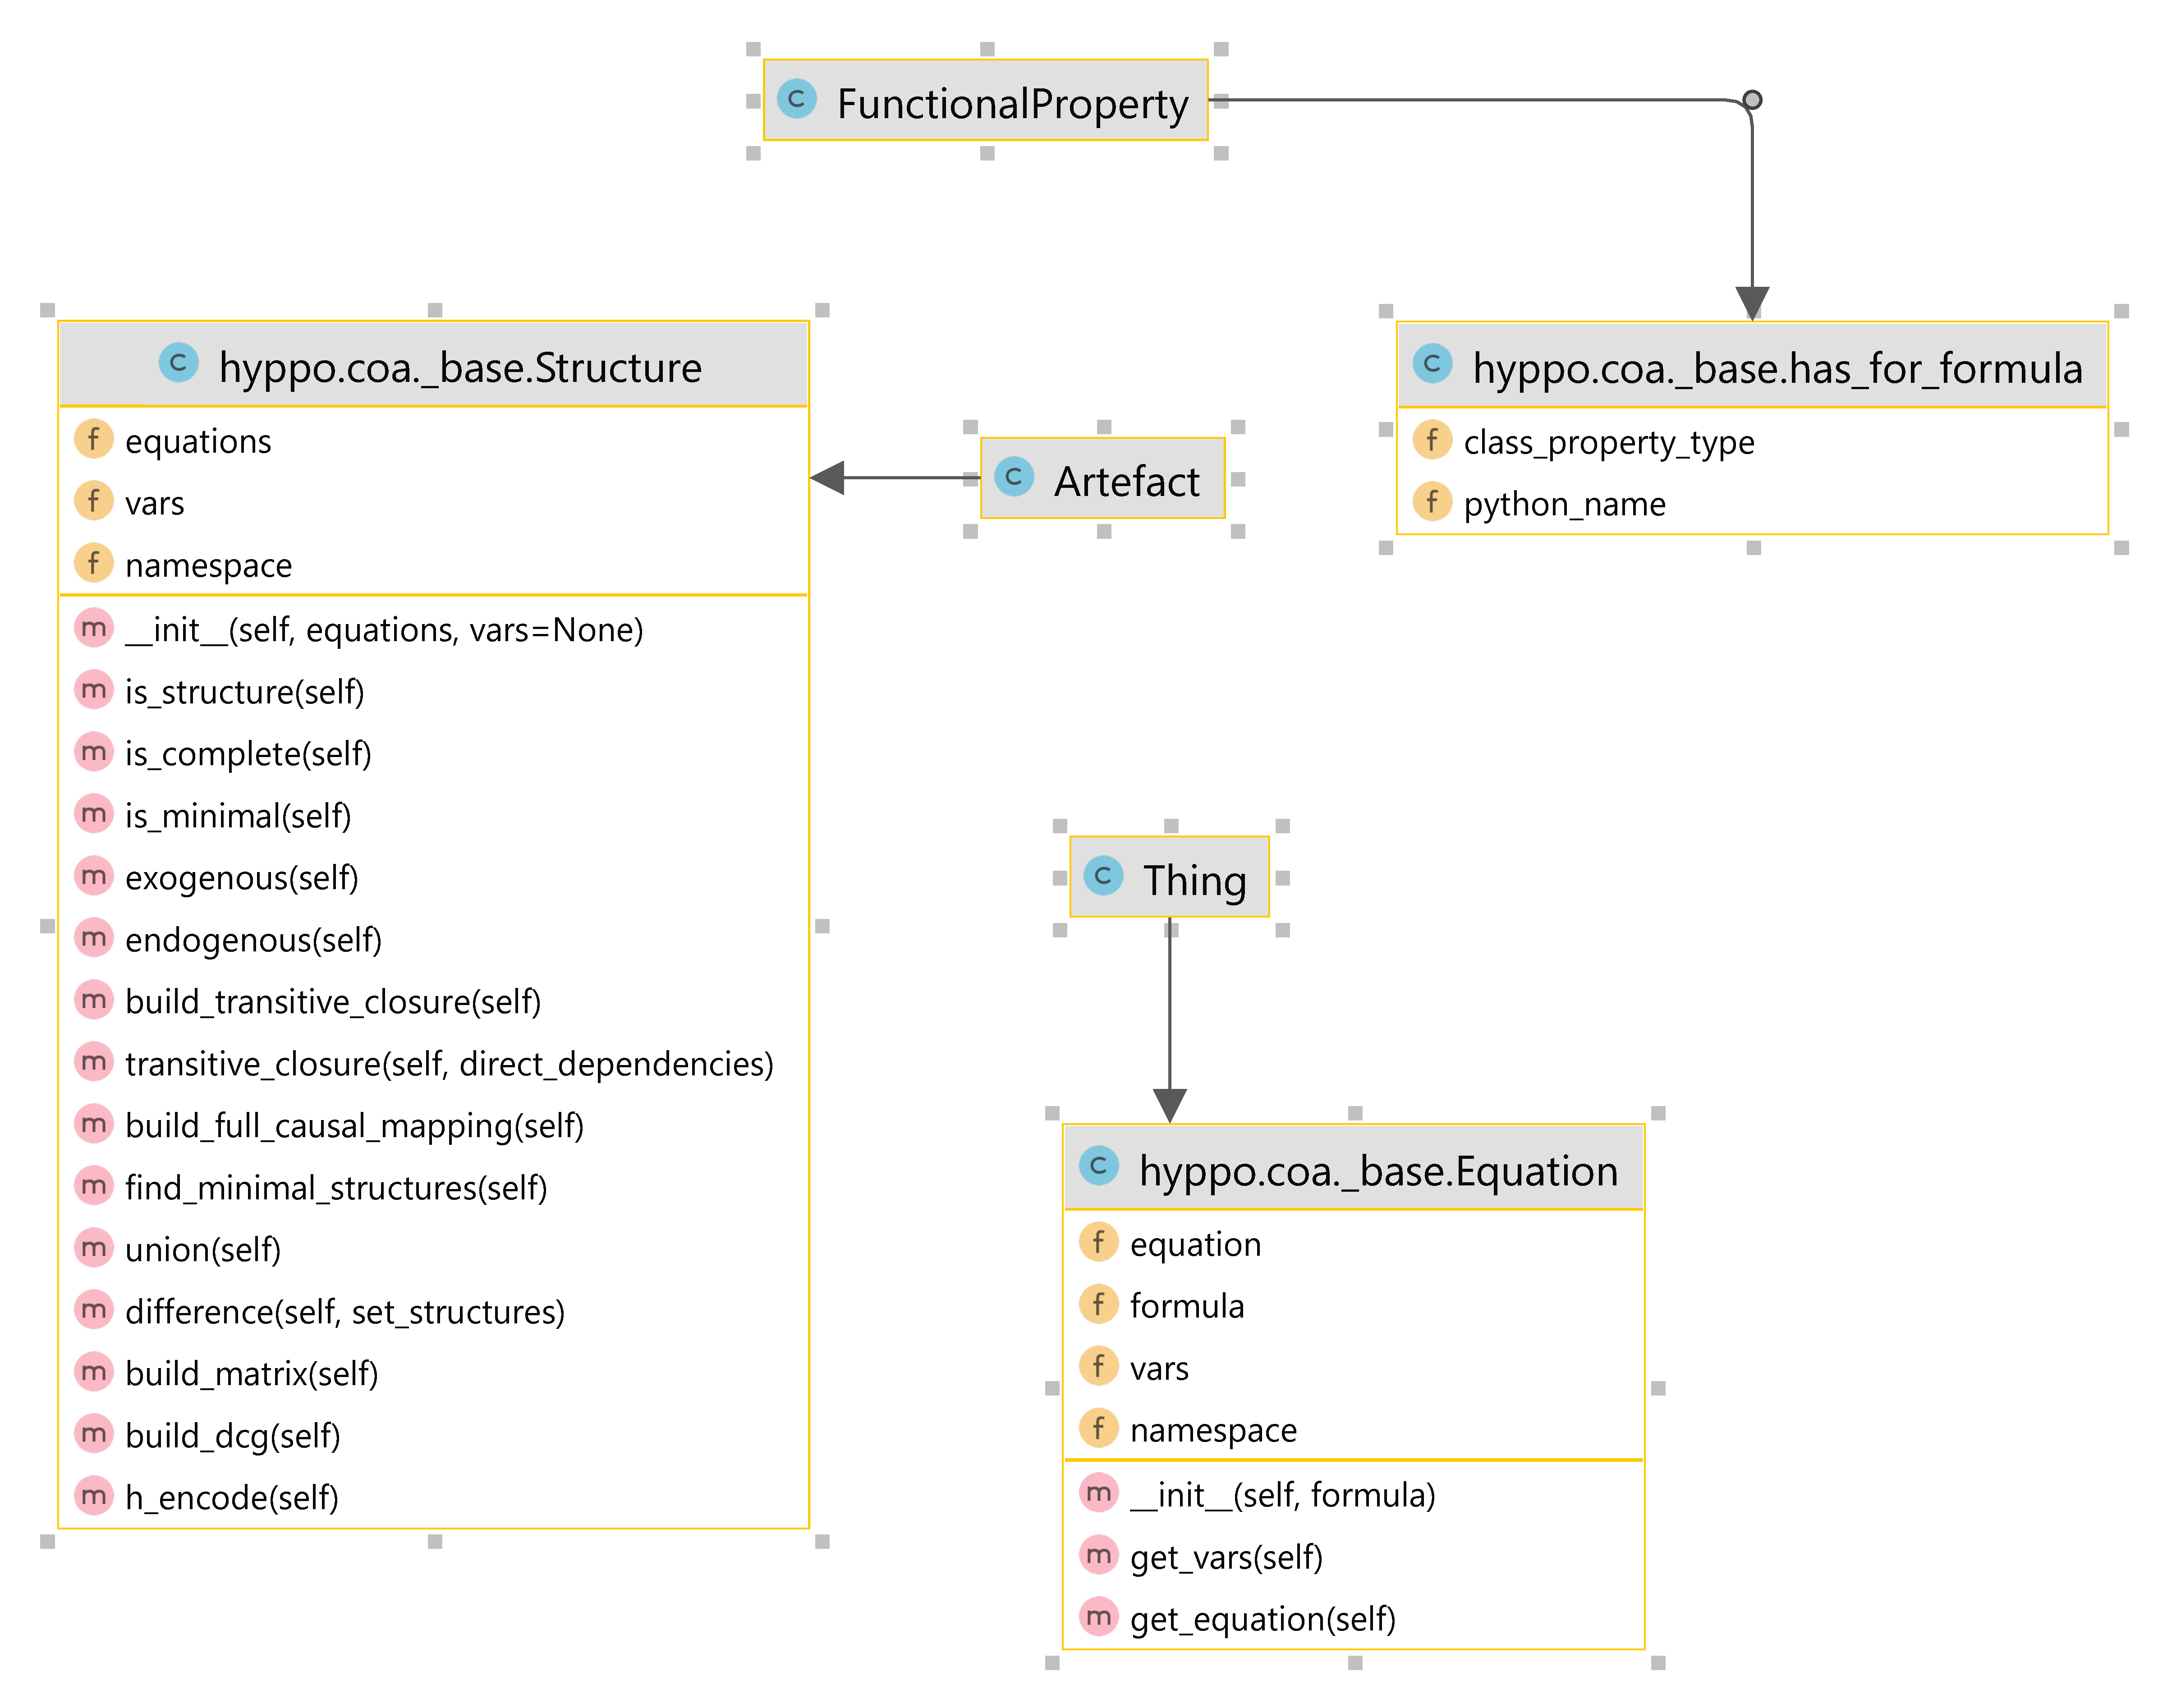
\includegraphics[width=0.9\linewidth]{images/base_coa.pdf}
    \caption{Диаграмма для пакета.}\label{fig:base_coa}
\end{figure}

Компонент включает в себя два класса \textbf{Equation} и \textbf{Structure}. Первый класс представляет собой класс 
уравнений, второй "--- класс структур. Для работы с уранениями и структурами используется их символьное представление.

Методы, входящие в класс \textbf{Equation}:
\begin{itemize}
    \item \textit{get\_vars(self)} "--- метод возвращает множество переменных уравнения.
    \item \textit{get\_equation(self)} "--- метод, преобразующий формулу LaTex в уравнение библиотеки SymPy.
\end{itemize}

Методы, входящие в класс \textbf{Structure}:
\begin{itemize}
    \item \textit{is\_structure(self)} "--- метод возвращает истину, если выполняется определение структуры, 
            иначе "--- ложь. 
    \item \textit{is\_complete(self)} "--- метод возвращает истину, если структура является полной, иначе "--- ложь. 
            Для этого проверяется равенство количества уравнений и количества переменных в структуре.
    \item \textit{is\_minimal(self)} "--- метод возвращает истину, если структура является минимальной, 
            иначе "--- ложь. Для этого проверяется полнота структуры и отсутствие минимальных структур, входящих в нее.
    \item \textit{exogenous(self)} "--- метод возвращает все экзогенные переменные, 
            принадлежащие множеству переменных структуры.
    \item \textit{endogenous(self)} "--- метод возвращает все эндогенные переменные, 
            принадлежащие множеству переменных структуры.
    \item \textit{build\_transitive\_closure(self)} "--- метод возвращает транзитивное замыкание для структуры. 
            Для этого сначала строится полное причинно-следственное отображение. Для каждой пары 
            уравнение-переменная из этого отображения для каждого уравнения извлекаются все его внутренние переменные 
            и удаляется внешняя переменная. Для оставшихся внутренних переменных формируются пары внутренняя 
            переменная - внешняя переменная. Все подобные пары добавляются в множество прямых причинно 
            следственных зависимостей, для которого строится транзитивное замыкание с использованием 
            метода \textit{deps\_transitive\_closure}.
    \item \textit{deps\_transitive\_closure(self, direct\_deps)} "--- метод возвращает транзитивное замыкание множества 
            прямых причинно следственных зависимостей. Для этого строится направленный граф, вершинами которого 
            являются переменные, а ребро из $x_a$ в $x_b$ существует, если во множество прямых зависимостей есть 
            соответствующая пара $(x_a, x_b)$. Далее для каждой вершины формируется пары, где первым элементом является 
            сама вершина, а вторым элементом "--- каждая вершина из множества достижимых вершин. Все пободные пары 
            добавляются в транзитивное замыкание.
    
    \item \textit{build\_full\_causal\_mapping(self)} "--- метод возвращает полное причинно-следственное отображение 
            для данной структуры. Последовательно происходит поиск минимальных подструктур, для которых добавляется 
            пара уравнение-переменные. После этого вычисляется разность между текущей структурой и минимальными и 
            описанная процедура повторяется.
    \item \textit{find\_minimal\_structures(self) } "--- метод возвращает для данной структуры все ее 
            минимальные подструктуры. Метод является рекурсивным. Для каждого элемента из множества всевозможных 
            подможеств подструктур проверяется, являются ли они минимальными. Если элемент является минимальной 
            структурой, то он добавляется в список возвращаемых структур.
    \item \textit{union(self, set\_structures)} "--- метод возвращает объединение структуры со множеством других 
            структур, подаваемых на вход. 
    \item \textit{difference(self, set\_structures)} "--- метод возвращает разность структуру и некоторого 
            множества структур $set\_structures$ . Так как структуры состоят из уравнений, а переменные являются 
            их частью только косвенно, как часть уравнений, соответственно разность вычисляется как разность на 
            множестве уравнений. После этого производится удаление переменных, принадлежащих 
            структурам из $set\_structures$.

    \item \textit{build\_matrix(self)} "--- метод возвращает структурную матрицу для данной структуры. 
            Построение происходит поэлементно, если переменная $x_j \in Vars(f_i)$, то $A_{ij} = 1$, иначе $0$.
    \item \textit{build\_dcg(self)} "--- метод возвращает направленный граф причинно-следственных зависимостей 
            переменных структуры в формате \texttt{dot}. 
    \item \textit{h\_encode(self)} "--- метод возвращает функциональные зависимости для данной структуры.

\end{itemize}



\subsection{Компонент построения решеток гипотез}\label{sect_4_2_3}

Компонент HypothesisLatticesConstructor обеспечивает автоматическое построение решеток гипотез по соответствующим 
им системам уравнений. Компонент загружает из базы данных метаинформации спецификацию потока работ и гипотез. 
Далее системы уравнений, соответствующих гипотезам, из спецификации переводятся во внутреннее представление, 
после чего вызывается компонент COAConstructor для построения причинно-следственного графа зависимостей переменных. 
Решетка гипотез сохраняется в базу данных метаинформации. Компонент реализован в виде модуля на языке Python с 
использованием библиотек pandas, numpy, itertools.
Методы, входящие в компонент:
\begin{itemize}
    \item \textit{build\_lattice(self)} "--- метод возвращает . 
    \item \textit{add\_hypothesis(self, hypothesis)} "--- метод возвращает истину, если структура является полной, 
            иначе "--- ложь. Для этого проверяется равенство количества уравнений и количества переменных в структуре.
    \item \textit{remove\_hypothesis(self, hypothesis)} "--- метод возвращает .
    \item \textit{derived\_by(self, hypothesis)} "--- метод возвращает .
    \item \textit{impacts(self, hypothesis)} "--- метод возвращает .
    \item \textit{is\_correct(self)} "--- метод возвращает .
    
\end{itemize}

Разработанный метод построения решеток гипотез реализован в виде отдельного компонента на языке Python 3.6 с 
использованием библиотеки для научных вычислений scipy и библиотеки поддержки многомерных массивов numpy. Компонент 
включает в себя функции загрузки спецификаций потока работ и гипотез, построения решетки гипотез по набору гипотез и 
потоку работ, вывод и сохранение результатов в локальную файловую систему. Входными данными для алгоритма являются 
спецификации потока работ и гипотез, загружаемые из локальной файловой системы. Реализация алгоритма построения 
решеток гипотез выполнена в отдельной функции, сохранение и отображение решетки гипотез также выполнено 
в отдельной функции.

\subsection{Планировщик виртуальных экспериментов}\label{sect_4_2_5}

Компонент VirtualExperimentPlanner вычисляет оптимальный план исполнения виртуального эксперимента, при этом 
используются решетки гипотез, содержащиеся в репозитории. Это позволяет до проведения виртуального эксперимента 
спланировать оптимальным образом подбор параметров гипотез и отсечь заранее непригодные комбинации параметров. 
Например, уже вычисленные результаты вызова функции модели могут быть повторно использованы в другом виртуальном 
эксперименте, а также могут помочь в исключении виртуального эксперимента, производящего данные, 
не совпадающие с реальными наблюдениями.

\subsubsection{Планирование виртуальных экспериментов}\label{sect_4_4}
Алгоритм планирования исполнения виртуальных экспериментов представлен в .

Использование в виртуальном эксперименте отдельных гипотез и соответствующих им моделей, а также оценка зависимостей 
гипотез друг от друга позволяет сохранять результаты выполнения отдельных частей виртуального эксперимента для их 
повторного использования. Это значительно увеличивает скорость исполнения виртуального эксперимента, повышая 
эффективность использования вычислительных ресурсов.

Основная идея метода повышения эффективности и скорости проведения виртуальных экспериментов состоит в следующем. 
На вход метод принимает спецификацию виртуального эксперимента и построенную для него решетку гипотез. Из множества 
гипотез виртуального эксперимента извлекаются конкурирующие гипотезы, т.е. те, для которых существует несколько 
возможных значений их параметров (гипотезы с разным значением одного параметра конкурируют друг с другом). 
Составляется сетка всевозможных комбинаций таких параметров. Далее с использованием решетки гипотез определяется 
порядок подстановки построенных комбинаций параметров в процессе исполнения виртуальных экспериментов. 
Данный процесс происходит итеративно, при этом на каждом шаге из решетки гипотез убираются гипотезы, не имеющие 
зависящих от себя других гипотез. Если для таких гипотез существуют конкурирующие, то подобная конфигурация 
параметров добавляется в план исполнения виртуального эксперимента. При этом те вызовы функций моделей, параметры для 
которых не изменились, считаются не требующими повторного вычисления, т.е. при непосредственном исполнении 
подставляется уже вычисленный фрагмент виртуального эксперимента. На выходе предоставляется план исполнения 
виртуального эксперимента с указанием порядка подстановки комбинаций параметров, а также частей виртуального 
эксперимента, требующих вызова функций моделей с новыми параметрами.

Метод применим как для работы с новым виртуальным экспериментом, так и для модифицированного виртуального 
эксперимента, например, после добавления в него нового значения параметров для существующей гипотезы. В первом 
случае будет возвращен план исполнения для всего эксперимента, тогда как во втором - только для новых комбинаций 
параметров. При изменении решетки гипотез или спецификации виртуального эксперимента данный метод в системе управления 
виртуальными экспериментами следует вызывать автоматически.
Алгоритм, реализующий разработанный метод, выполнен на языке Python 3.6 с использованием библиотек NumPy, SciPy, 
Pandas. Реализация выполнена в виде отдельного модуля. Для хранения результатов проведенных экспериментов используется 
реляционная база данных.


\subsubsection{Отказ от некоторых вычислительных маршрутов}\label{sect_4_3}



\subsection{Компонент исполнения виртуальных экспериментов}\label{sect_4_2_6}

Компонент VirtualExperimentRunner запускается для непосредственного исполнения виртуального эксперимента. 
Из репозитория метаинформации загружаются спецификация виртуального эксперимента и дополнительно построенные 
решетка гипотез и план исполнения виртуального эксперимента. Исполнение происходит в соответствии с планом, при 
этом система использует сохраненные результаты исполнения части виртуального эксперимента (при их наличии в 
репозитории метаинформации). Используя спецификацию моделей виртуального эксперимента, компонент осуществляет 
вызов соответствующих функций, а затем собирает полученные данные от них. Результаты исполнения виртуального 
эксперимента сохраняются в базу данных метаинформации.


\subsection{Репозиторий метаинформации}\label{sect_4_2_7}

\begin{figure}[h!]
    \centering
    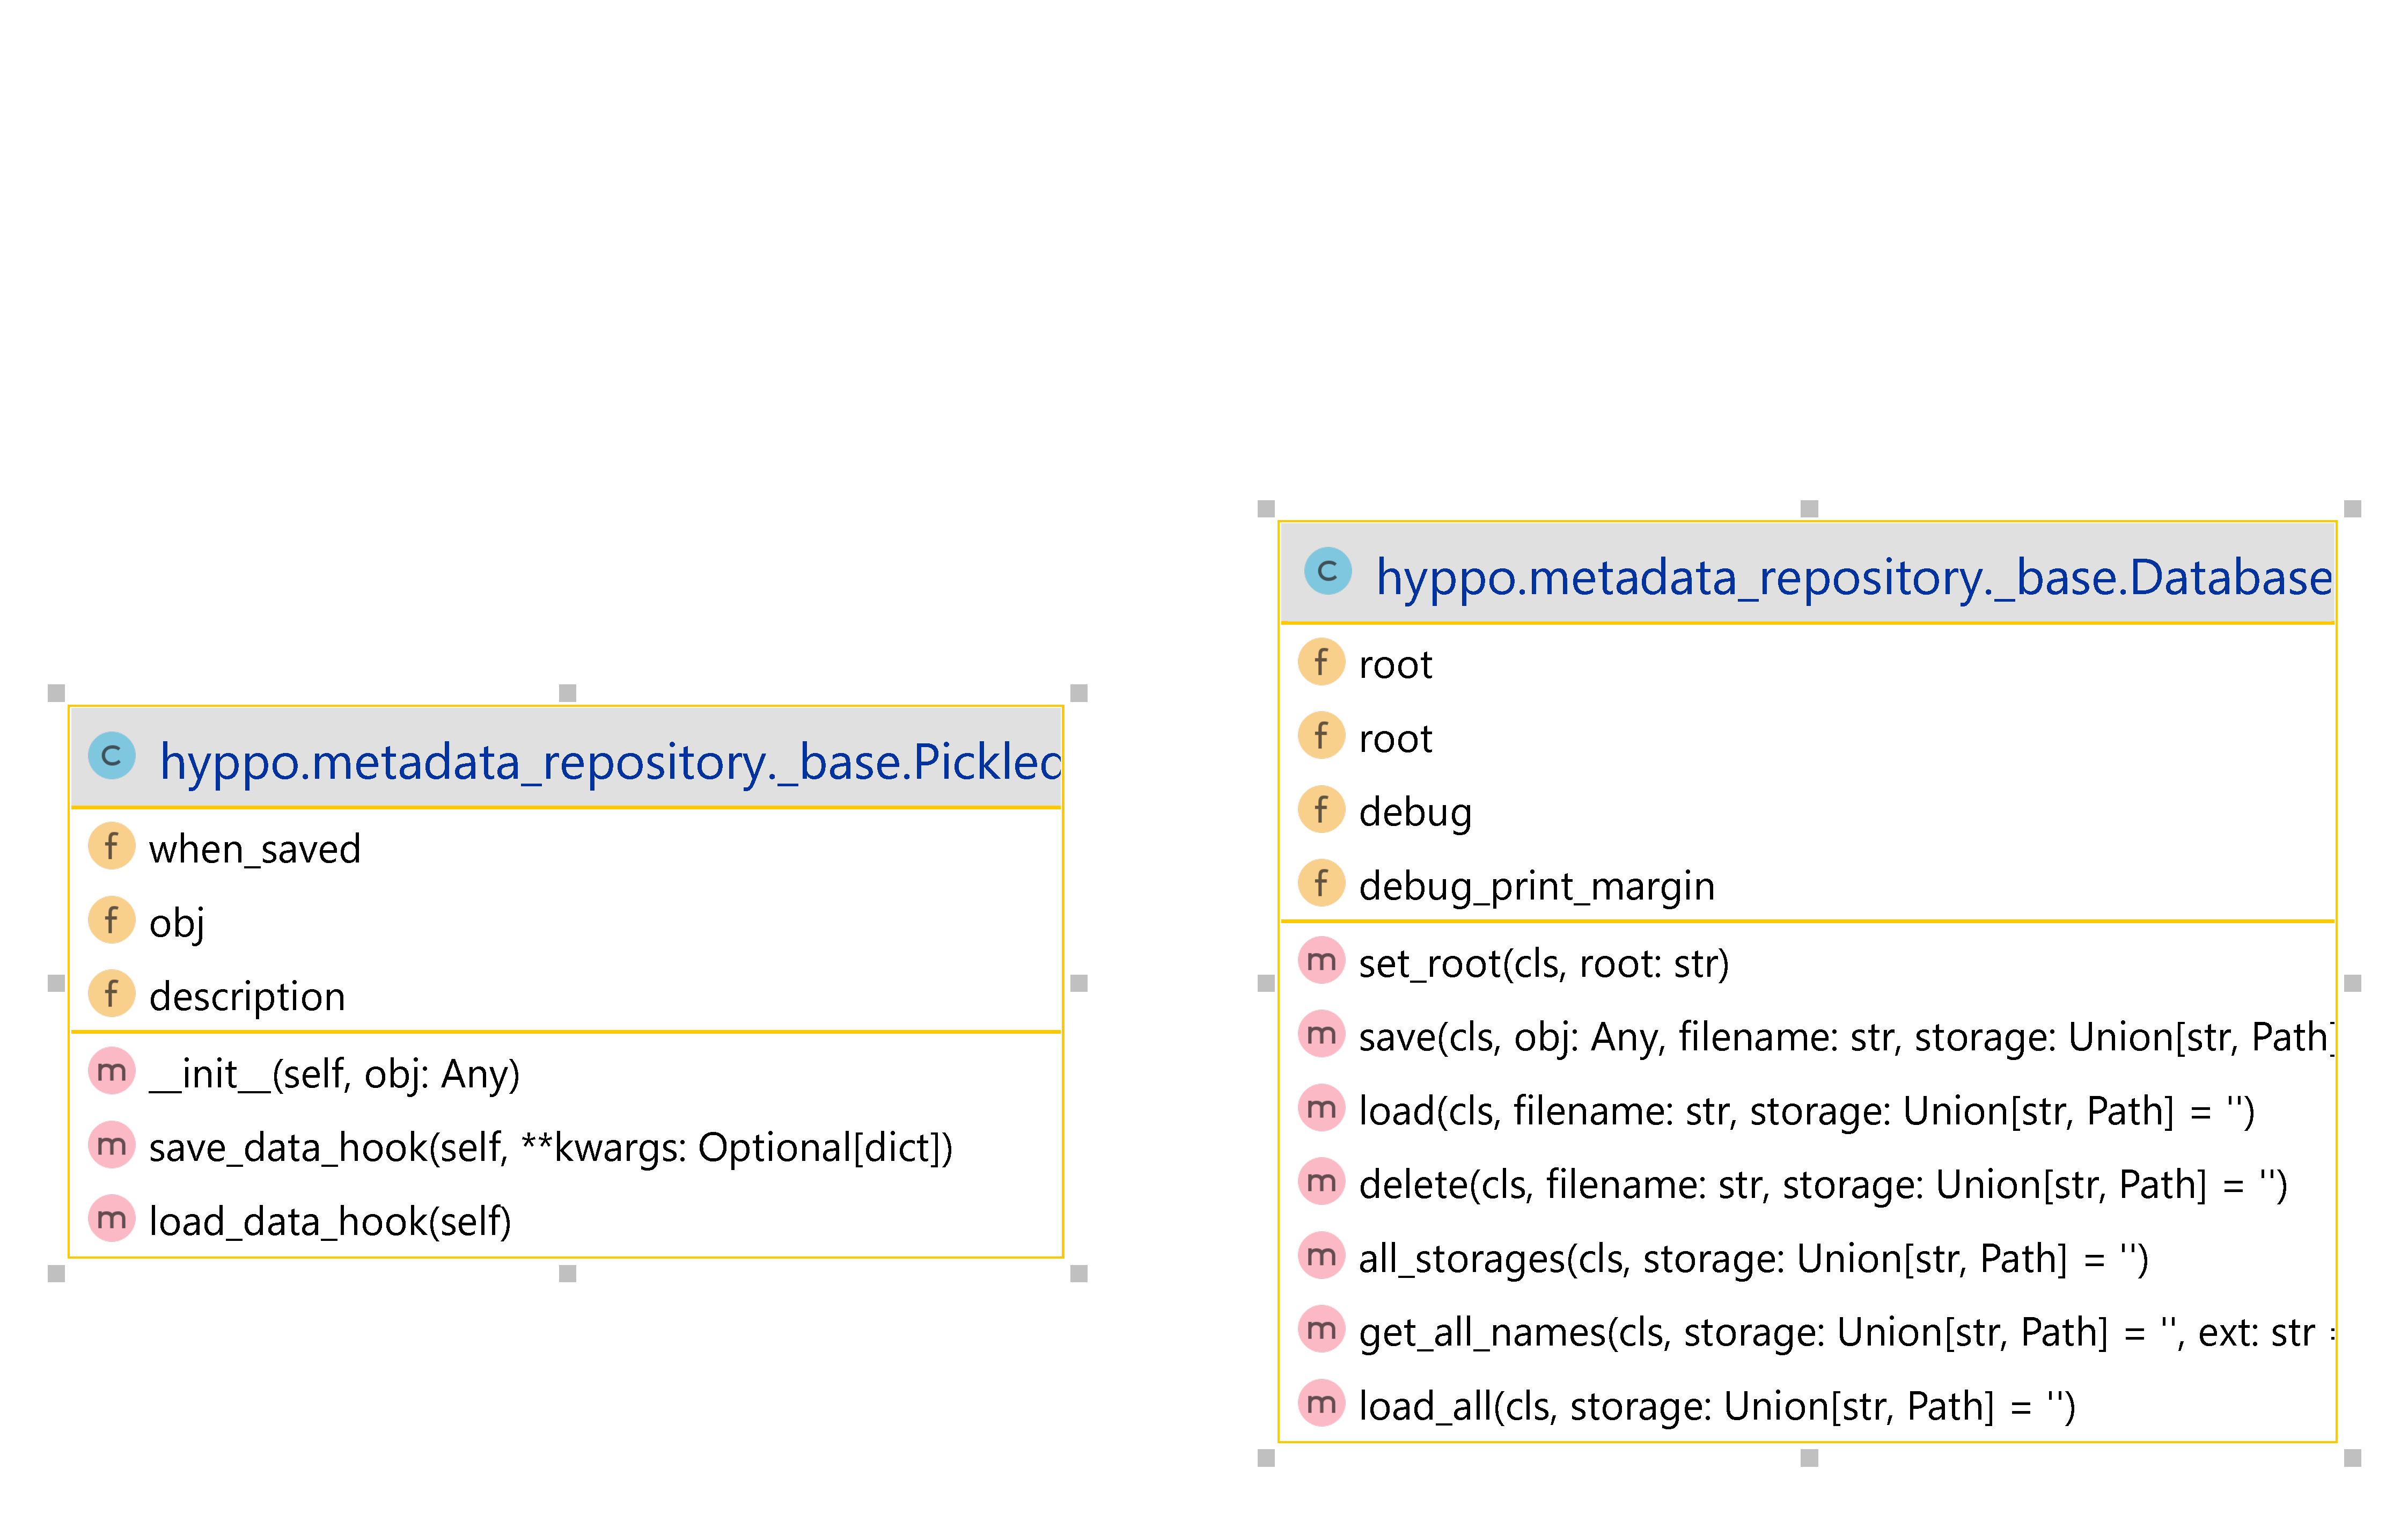
\includegraphics[width=0.9\linewidth]{images/_repo.pdf}
    \caption{Диаграмма для пакета.}\label{fig:repo}
\end{figure}
\cref{fig:repo}

%\section{Поиск оптимальных параметров гипотез}\label{sect_4_5}
\section{Инфраструктура для работы с платформой}\label{sect_4_5}

\subsection{Аппаратное и программное обеспечение кластера}\label{sect_4_5_1}

Эксперименты по адаптации программной реализации нейросетевых моделей для выполнения в распределенной 
вычислительной среде были проведены с использованием прототипа вычислительного кластера. Кластер включает в 
себя главный узел и четыре вычислительных узла и развернут как часть инфраструктуры совместных исследовательских 
объектов для высокопроизводительных вычислений ФИЦ ИУ РАН. Аппаратная архитектура кластера показана на 
\cref{fig:lab_cluster}. Вычислительные узлы включают в себя два процессора Intel Xeon 2630L с частотой 2,5 ГГц и 
24 виртуальными ядрами, 64 ГБ оперативной памяти DDR3 1066 МГц, один твердотельный накопитель емкостью 160 Гб и 
четыре жестких диска емкостью 2 ТБ каждый. Кластер также включает файловый сервер Quanta Stratos S810 с двумя 
процессорами Intel XEON 2670, 96 ГБ оперативной памяти DDR3 1066 МГц, один твердотельный накопитель INTEL S3500 
емкостью 480 ГБ, RAID-массив, состоящий из 15 жестких дисков по 2 ТБ каждый, и RAID-массив, состоящий из 
8 твердотельных накопителей INTEL S3500 емкостью 480 ГБ каждый. Сеть Ethernet поддерживается коммутатором 
Quanta LB6M 10GbE.

\begin{figure}[h!]
    \centering
    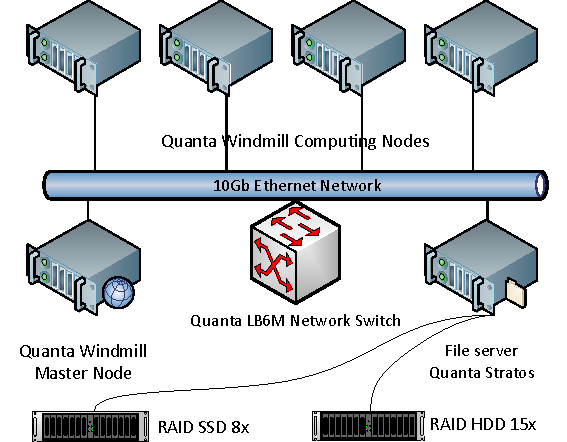
\includegraphics[width=0.7\linewidth]{images/lab_cluster.pdf}
    \caption{Инфраструктура платформы исполнения виртуальных экспериментов.}\label{fig:lab_cluster}
\end{figure}

На кластере установлена платформа данных Hortonworks с открытым исходным кодом 3.1.4.0 \cite{HDP2021}, 
предназначенная для распределенных вычислений. Платформа основана на платформе распределенного управления 
данными Hadoop \cite{hadoop} и файловой системе HDFS \cite{borthakur2007hadoop}. В частности, платформа включает 
в себя систему управления ресурсами YARN и планирования/мониторинга заданий, а также систему обработки данных Spark, 
предназначенную для распределенного использования общей памяти. 

Распределенная файловая система HDFS устанавливается поверх файловой системы Linux ext3. Файлы хранятся в HDFS в 
виде наборов блоков определенного размера. Разные блоки одного и того же файла могут храниться на разных узлах 
кластера. Блоки файлов реплицируются для обеспечения отказоустойчивости. Несколько реплик блока хранятся на разных 
узлах кластера. Репликация блоков "--- это автоматическая процедура: если файловый блок поврежден, автоматически 
используется реплика. HDFS масштабируется по объему данных: новые узлы могут добавляться в кластер динамически. 

YARN разделяет управление ресурсами и планирование заданий/мониторинг на отдельные демоны: global ResourceManager и 
ApplicationMaster. Экземпляр ApplicationMaster создается для каждого приложения. ResourceManager и NodeManager 
формируют структуру вычислений данных. ResourceManager управляет ресурсами между всеми приложениями в системе. 
Для каждого приложения выделяется контейнер, а также права на использование заданного объема ресурсов (процессор, 
память, диск, сеть). NodeManager - это агент узла для каждого кластера, отвечающий за контейнеры, отслеживающий 
использование их ресурсов и сообщающий об этом ResourceManager. ApplicationMaster согласовывает ресурсы с 
ResourceManager и работает с NodeManager для выполнения и мониторинга задач.

YARN позволяет развертывать различные фреймворки для распределенной обработки данных в кластере Hadoop, такие как 
MapReduce для пакетной обработки, Tez для моделирования обработки данных в виде графика потока данных, Storm 
для потоковой обработки и так далее. 

Spark \cite{zaharia2010spark} - одна из самых популярных систем обработки данных для Hadoop. Spark предназначен 
для хранения и обработки данных в распределенной общей памяти, повышающей производительность при решении различного 
рода задач. Spark особенно полезен для распределенного машинного обучения с итеративными алгоритмами, посещающими 
наборы данных несколько раз в цикле. Архитектурной особенностью Spark является устойчивый распределенный набор 
данных (RDD), доступный только для чтения мультинабор элементов данных, распределенных по кластеру машин, 
который поддерживается отказоустойчивым способом. RDDS можно манипулировать с помощью различных параллельных операций.

Приложения Spark, называемые драйверами, выполняются как независимые наборы процессов в кластере, координируемые 
объектом SparkContext. SparkContext может подключаться к нескольким типам менеджеров кластеров (например, YARN), 
которые распределяют ресурсы между приложениями. После установления соединения Spark получает исполнителей на 
рабочих узлах кластера, которые представляют собой процессы, выполняющие вычисления и хранящие данные для 
приложения. Код приложения, определенный файлами JAR или Python, передается в SparkContext. Наконец, 
SparkContext отправляет задачи исполнителям для выполнения.

Прототип кластерного программного обеспечения ориентирован на развертывание на платформах облачных вычислений. 
Все программные компоненты инкапсулированы в контейнеры системы виртуализации уровня ОС с открытым 
исходным кодом Docker \cite{anderson2015docker}.

\subsection{Базовое программное обеспечение для запуска платформы на кластере}

Взаимодействие платформы и кластера приведено на \cref{fig:platform_cluster}.

\begin{figure}[h!]
    \centering
    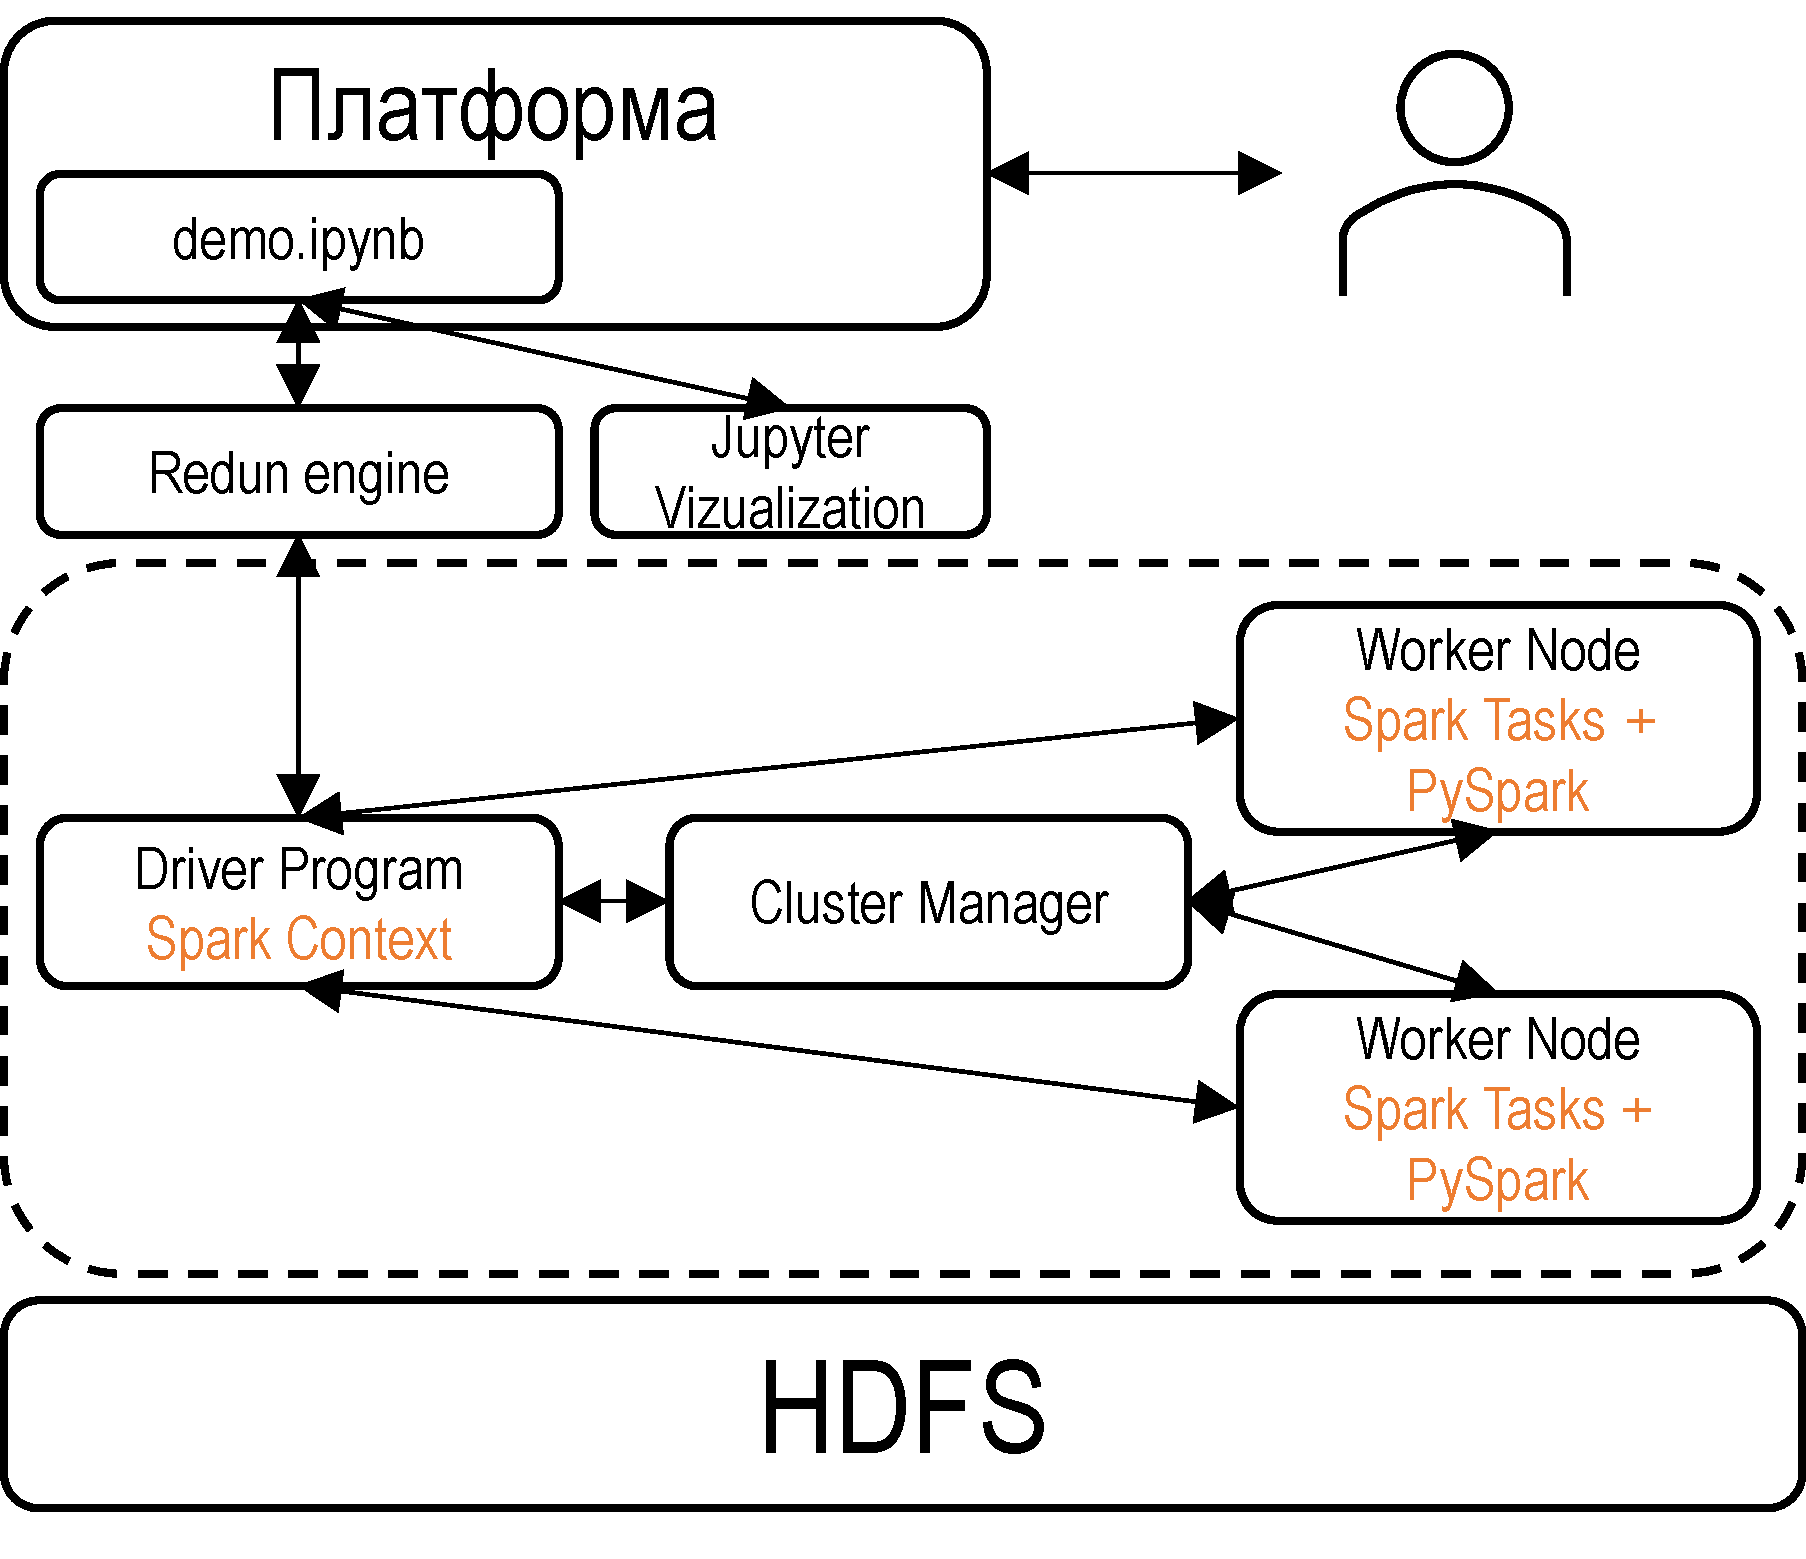
\includegraphics[width=0.7\linewidth]{images/platform_cluster.pdf}
    \caption{Запуск примера с использованием Платформы на кластере.}\label{fig:platform_cluster}
\end{figure}


Nibabel \cite{gorgolewski2011nipype} "--- это библиотека, предоставляющая API для чтения и записи 
некоторых распространенных форматов файлов для нейровизуализации. Эти форматы включают: ANALYZE (обычный, 
SPM99, SPM2 и выше), FIFTY, Nifty 1, Nifty 2, MINS1, MINS2, MGH и EAT, а также Philips PAR/REC. Различные 
классы форматов изображений обеспечивают полный или выборочный доступ к информации заголовка (meta), а 
доступ к данным изображения предоставляется через массивы библиотеки numpy.

Объекты изображения Nibabel состоят из трех элементов:
\begin{enumerate}
    \item $n$-мерный массив, содержащий изображение.
    \item Матрица аффинных преобразований размером 4х4, которая соотносит координаты изображения 
            со стандартным мировым координатным пространством.
    \item Метаданные изображения, хранящиеся в заголовке.
\end{enumerate}

При загрузке изображения создается объект типа Nifti1image. Имя файла может иметь расширение  .nii или .nii.gz. 

Стоит отметить, что при непосредственном вызове функции загрузки данные изображения не загружаются в память, 
поскольку изображения могут храниться в виде массива numpy на диске. Чтобы загрузить данные с диска,  необходимо 
вызвать функцию $get\_data()$ объекта типа Nifti1Image. Эта функция возвращает $n$-мерный массив numpy. Кроме того, 
объект типа Nifti1Image создается из массивов numpy. Чтобы сделать это, необходимо передать $n$-мерный массив данных 
и матрицу аффинного преобразования конструктору Nifti1Image.

Nitime \cite{rokem2009nitime} "--- это библиотека для анализа временных рядов в области нейровизуализации. 
Nitime может использоваться для представления, обработки и анализа данных временных рядов на основе экспериментальных 
данных. Основная цель библиотеки - служить платформой для анализа данных, собранных в ходе нейрофизических 
экспериментов. Основным принципом реализации nitime является разделение представления временных рядов и 
анализа временных рядов.

Важной особенностью библиотеки anytime является отложенная инициализация. Большинство атрибутов как временных 
рядов, так и объектов анализа используются только при необходимости. То есть инициализация объекта временного 
ряда или объекта анализа не вызывает каких-либо интенсивных вычислений. Кроме того, после запуска вычисления 
объект сохраняется и гарантирует, что доступ к результатам анализа приведет к выполнению вычисления только при 
первом выполнении анализа. После этого результат анализа сохраняется для дальнейшего использования. Одним из 
алгоритмов библиотеки nitime является корреляционный анализ областей мозга. Он вычисляет корреляцию между одним 
временным рядом, представляющим данную область мозга, и другими областями, которые также представлены временным 
рядом. Для вычисления корреляции между регионами в библиотеке nitime существует функция SeedCoherencAnalyzer, 
которая принимает два входных данных временных рядов и возвращает корреляционную матрицу, которую можно 
использовать для дальнейшего анализа.

Nilearn \cite{abraham2014machine} "--- это модуль Python для статистической обработки данных нейровизуализации.
Он использует модуль scikit-learn для многомерной статистики с приложениями для интеллектуального моделирования, 
классификации, декодирования и анализа связности. Nilearn может работать с объектами NiftiImage из библиотеки nibabel.
Библиотека Nilearn обладает большой функциональностью для работы с nii-изображениями. Это позволяет визуализировать, 
декодировать, исследовать функциональную связность и выполнять различные манипуляции, такие как сглаживание, 
маркировка и расширенный статистический анализ.
Nilearn предоставляет метод CanICA, который является методом ICA для анализа данных МРТ на групповом уровне. 
По сравнению с другими стратегиями, это обеспечивает хорошо контролируемую групповую модель, а также пороговый 
алгоритм, который контролирует специфичность и чувствительность с помощью явной модели сигнала. 
Чтобы получить временной ряд и построить для него корреляционную матрицу, nilearn предоставляет объект NiftiMapsMasker. 
Чтобы создать объект, нужно указать атлас областей мозга. Nilearn предоставляет возможность создавать корреляционную 
матрицу для независимых компонентов, которая вычисляется CanICA.

Программа считывает все файлы из каталога, проверяет правильность формата (все данные сжаты). После этого номер темы 
извлекается из имени файла и его пол проверяется с помощью дополнительного файла метаданных. Когда пол известен, файл 
распаковывается в соответствующую папку. Внутри распакованной папки находится 4-D изображение в .nii.gz формат. 
Используя библиотеку nibabel, изображение загружается в память в виде массива типа numpy.array. Из этого массива 
создается новый массив с информацией о пространственных координатах перед значением вокселя. Новый массив с
жимается с помощью алгоритма gzip и сохраняется в HDFS.

Задачи Spark запускаются со следующими параметрами:
\begin{itemize}
    \item \textit{num-исполнитель = 4} - количество исполняемых объектов.
    \item \textit{executor-memory = 25GB} - объем памяти, используемый для одного процесса выполнения.
    \item \textit{executor-cores = 2} - количество ядер, используемых для каждого исполнительного объекта.
    \item \textit{driver-memory = 8GB} - объем памяти, используемый для процесса драйвера.
\end{itemize}

\section{Выводы по главе}\label{sect3_3}
\clearpage
